\section{Lexer}
The handed out Lexer has been extended as to acommodate for other operators, the implementation of which has also been made elsewhere.
The purpose of the lexer is to recognize our input and "parse" properly to the parser, such that input be distinguished and handled properly.\\
The lexer matches token which include keywords and operators. Keywords are proper "words" like function-names, variables and statements like \textit{if-then-else}-statements.\\
Operators on the other hand are things like \textit{+,-,\&\& etc.}. Both of these, when written, will be recognized by the lexler and passed approriately to the parser like so:\\
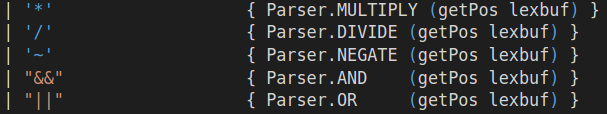
\includegraphics[width=\linewidth]{Materials/Lexer/Lexer}
